% ============================================================================
% LaTeX Research Proposal Template
% Created by: Aatiz Ghimire
% Institution: Tribhuvan University, Institute of Science and Technology
% Version: 1.0
% Date: December, 2024
% Description: Template for research proposals based on the required structure.
% License: Open for use by students of Tribhuvan University with appropriate credit.
% ============================================================================

\documentclass[12pt, a4paper]{report}

% Packages
\usepackage{graphicx} % For including images
\usepackage{geometry} % For customizing margins
\usepackage{setspace} % For line spacing
\usepackage{times}    % Times New Roman font for PDFLaTeX
\usepackage{parskip}  % Better control over paragraph spacing
\usepackage{titlesec} % For customizing headings
\usepackage{caption}  % For customizing figure and table captions
\usepackage{amsmath}  % For mathematical equations
\usepackage{amssymb}  % For additional math symbols
\usepackage{array}
\usepackage{pgfgantt}
\usepackage{xcolor}
\usepackage{booktabs}
\usepackage{adjustbox}
\usepackage{ragged2e}
\usepackage{longtable}
\bibliographystyle{IEEEtran}

% === COLORS ===
\definecolor{task1}{RGB}{255, 140, 0}   % orange!70
\definecolor{task2}{RGB}{0, 128, 128}   % teal!50
\definecolor{task3}{RGB}{34, 139, 34}   % green!60
\definecolor{task4}{RGB}{199, 21, 133}  % magenta!50
\definecolor{task5}{RGB}{255, 215, 0}   % yellow!70
\definecolor{task6}{RGB}{128, 0, 128}   % purple!60

% Page Margins
\geometry{
    a4paper,
    top=1cm,
    bottom=1.5cm,
    left=2cm,
    right=2cm
}

% Line Spacing
\setstretch{1.5}  % Set line spacing to 1.5

% Paragraph Formatting
\setlength{\parindent}{1.5em}  % Indentation for paragraphs

% Heading Styles
\titleformat{\chapter}[block]{\bfseries\fontsize{16}{20}\selectfont}{\thechapter.}{0.3em}{}
\titlespacing*{\chapter}{0pt}{0pt}{0pt}
\titleformat{\section}[block]{\bfseries\fontsize{14}{18}\selectfont}{\thesection}{0.3em}{}
\titleformat{\subsection}[block]{\bfseries\fontsize{12}{16}\selectfont}{\thesubsection}{0.3em}{}

% Caption Styles
\captionsetup[figure]{
    font={bf,small},
    labelfont={bf},
    justification=centering,
    labelsep=colon,
    textfont=bf
}
\captionsetup[table]{
    font={bf,small},
    labelfont={bf},
    justification=centering,
    labelsep=colon,
    textfont=bf,
    position=above
}

% Document Starts
\begin{document}

% Title Page
\begin{titlepage}
    \begin{center}
        
\includegraphics[width=0.2\textwidth]{logo.png}\\[0.5cm] % Replace with the actual logo file path
        \vspace{0.5cm}
        
        {\Large \textbf{Chittagong University of Engineering and Technology}}\\
        {\Large \textbf{Department of Computer Science and Engineering}}\\[1.0cm]

        {\large \textbf{A Research Proposal on}}\\

        {\Large \textbf{Explainable HybridNet: A Lightweight CNN–Transformer Framework for Intelligent DDoS Attack Detection and Interpretation in Modern Networks}}

        \textbf{Submitted by}\\
        {\large \textbf{Kazi Nazmul Hasan}}\\
        \textbf{ID: 23MCSE725}\\[1cm]

        \textbf{Under the Supervision of}\\
        { \Large\textbf{Prof. Dr. Mohammad Shamsul Arefin}}\\
        {\textbf{Department of Computer Science and Engineering}}\\
         { \textbf{Chittagong University of Engineering and Technology}}\\

        % \textbf{Submitted to}\\
        % {\large \textbf{School of Mathematical Sciences}}\\
        % {\large \textbf{Kirtipur, Kathmandu, Nepal}}\\[1cm]

        % \textbf{Submitted in partial fulfillment of the requirements for the degree of Master in Data Science}\\[2cm]

        % \textbf{[Month, Year]}\\
    \end{center}
\end{titlepage}


% Table of Contents
\tableofcontents

% Roman Page Numbering for ToC and Preliminary Sections
\pagenumbering{roman}
\pagestyle{plain}

\clearpage

%%%%%%%%%%%%%%%%%%%%%%% Chapter 1: Introduction %%%%%%%%%%%%%%%%%%%%%%%%%%%%%
\chapter{Introduction}
In recent years, the explosive growth of Internet‑connected devices and cloud‑based applications has significantly increased the attack surface of modern networks. Among all cyber threats, Distributed Denial of Service (DDoS) attacks remain one of the most disruptive and frequent, capable of paralyzing large‑scale systems, degrading service quality, and causing financial and reputational loss. Traditional intrusion detection systems (IDS) — whether signature‑based or rule‑based — struggle to cope with the dynamic, high‑volume, and evolving nature of modern DDoS traffic.

To overcome these limitations, the research community has shifted toward machine learning (ML) and deep learning (DL)‑based network intrusion detection systems (NIDS). Deep Convolutional Neural Networks (CNNs) have shown remarkable success in learning spatial feature representations from network traffic \cite{1mohammadpour2022cnn_ids}. Meanwhile, Transformers, originally designed for Natural Language Processing (NLP), have recently proven effective in capturing temporal and contextual relationships in sequential network data \cite{2farias2025transformers_ddos}. However, most existing DL‑based models for DDoS detection are computationally expensive, non‑explainable, and unsuitable for real-time deployment on edge or IoT environments.



\pagestyle{plain} % Default style for numbered pages
\pagenumbering{arabic} % Start Arabic numbering from here

\section{The Problem or Issue Being Addressed}


Despite advances in deep learning, several challenges persist in building lightweight and interpretable models for DDoS detection:
\begin{itemize}
  

 \item The high computational cost of Transformer-based architectures limits deployment in low-resource environments \cite{3wang2024ddos_msct}.

 \item Lack of explainability makes it difficult for analysts to understand why a model flags certain traffic as malicious, reducing trust in automated security systems \cite{4zhang2025intrusion_cnn_bilstm_transformer}.

 \item Limited scalability in real-time traffic monitoring scenarios, especially when dealing with high throughput and diverse attack patterns \cite{5liu2025cnn_lstm_transformer_ids}.
\end{itemize}
Therefore, there is a clear need for a framework that can efficiently detect DDoS attacks in real time, while also providing interpretable explanations for its decision
\section{Rationale: Why This Research Is Important}
The proposed research, Explainable HybridNet, addresses these challenges by integrating the strengths of CNNs (for feature extraction) and Transformers (for contextual understanding) into a hybrid lightweight model optimized for real-time network intrusion detection.

Key motivations include:
\begin{itemize}
   

 \item Performance–Efficiency Balance: Designing a compact model architecture that maintains high detection accuracy while minimizing computational and memory overhead \cite{6alzahrani2024lightweight_cnn_lstm_ids}. However, a persistent challenge remains in balancing these optimization levels with the complex spatial-temporal feature requirements of modern DDoS attacks \cite{deng2020model}.

 \item Transparency in AI: Embedding explainability modules to help cybersecurity analysts interpret model outputs, improving trust, accountability, and compliance with emerging AI regulations \cite{7harshdeep2025deeptransids}.

 \item Practical Deployment: Enabling edge and IoT network security monitoring with low latency and energy-efficient inference \cite{8alzu’bi2024explainable_ai_ddos}.
\end{itemize}
 \item Contribution to Modern Network Security: Providing a benchmark framework and reproducible design for future research in explainable, resource-efficient AI-based security systems \cite{9shaikh2024advancing_ddos_hybrid}.
\section{Scope and Limitations}
\textbf{Scope:}
\begin{itemize}
 
\item Focuses on DDoS attack detection using network flow-based features (not payload-level inspection)~\cite{10kamal2024advanced_hybrid_transformer_cnn}.
    \item Utilizes publicly available datasets such as CIC-DDoS2019, CSE-CIC-IDS2018, CICIoT2023, and Edge-IIoTset for training and evaluation~\cite{11liu2025ensemble_xai_ids}\cite{12Wahab2025}\cite{neto2023ciciot2023}\cite{ferrag2022edge}.
    \item Incorporates explainable AI (XAI) techniques (e.g., attention visualization, SHAP-based interpretation) for interpretability.
    \item Targets real-time and edge deployment, emphasizing low-latency inference and lightweight architecture design. 
\end{itemize}

    \textbf{Limitations:}
    \begin{itemize}
    \item The model may not detect zero-day attacks beyond learned traffic patterns without retraining or online adaptation.
    \item Explainability may be approximate due to reduced computational complexity in lightweight XAI methods.
    \item Experiments are limited to synthetic and benchmark datasets; real-world validation will require future deployment studies.
    \item The research does not focus on other attack types such as data exfiltration or insider threats.
\end{itemize}
% \subsection{Research Questions}
% What are the comparative advantages and limitations of classical, neuromorphic, and quantum models in terms of performance and scalability?

%%%%%%%%%%%%%%%%%%%%%%% Chapter 2: literature  %%%%%%%%%%%%%%%%%%%%%%%%%%%%%
\chapter{Literature Review}
\small
\begin{table*}
\centering
\small
\caption{Comparison Chart of Studies on DDoS Detection using DL and Hybrid Models}
\label{tab:comparative-study}
\begin{adjustbox}{max width=\linewidth}
\begin{tabular}{
  >{\RaggedRight}p{0.13\linewidth}
  >{\RaggedRight}p{0.16\linewidth}
  >{\RaggedRight}p{0.12\linewidth}
  >{\RaggedRight}p{0.20\linewidth}
  >{\RaggedRight}p{0.07\linewidth}
  >{\RaggedRight}p{0.25\linewidth}
}
\toprule
\textbf{Study} & \textbf{Algorithm / Method} & \textbf{Dataset} & \textbf{Result} & \textbf{Acc.} & \textbf{Research Gaps / Notes} \\
\midrule
Sathaporn et al. \cite{13Sathaporn2025} & CNN-RNN + Multi-Head Attention & Cloud network traffic & High DDoS detection, low false positives & 95\% & Not lightweight, limited interpretability \\
\midrule
Zhang et al. \cite{4zhang2025intrusion_cnn_bilstm_transformer} & CNN-BiLSTM-Transformer & CIC-IDS2018 & Improved sequential attack detection & 94\% & High computation, real-time deployment challenge \\
\midrule
Muhammet and Polat \cite{yagiz2025lensxai} & Knowledge Distillation + VAE & IIoT Gateways & Scalable attribution-based XAI & 93\% & Focuses on IIoT; lacks heavy traffic benchmark \\
\midrule
Liu et al. \cite{5liu2025cnn_lstm_transformer_ids} & CNN-LSTM-Transformer & NSL-KDD & Better temporal feature learning & 93\% & Non-explainable, high resource usage \\
\midrule
Shaikh, 2024 \cite{9shaikh2024advancing_ddos_hybrid} & CNN + PCA + Vision Transformer & CIC-DDoS2019 & High DDoS detection accuracy & 96\% & Lacks lightweight model for edge devices \\
\midrule
Long et al., 2024 \cite{14Long2024} & Transformer & Cloud traffic & Accurate detection for cloud attacks & 92\% & Heavy computation, not real-time \\
\midrule
Wang, 2024 \cite{3wang2024ddos_msct} & Multi-scale CNN + Transformer & CIC-DDoS2019 & Efficient multi-class detection & 94\% & Slightly complex; limited XAI \\
\midrule
Alabdulatif et al., 2025 \cite{15Alabdulatif2025} & Ensemble DL + XAI & CSE-CIC-IDS2018 & Explainable detection, high accuracy & 95\% & Large model; edge deployment limited \\
\midrule
Alzahrani, 2024 \cite{6alzahrani2024lightweight_cnn_lstm_ids} & CNN-LSTM & IoT traffic & Lightweight, faster inference & 90\% & Limited interpretability; attack type coverage \\
\midrule
Harshdeep, 2025 \cite{16Harshdeep2025} & Transformer & 5G IoT traffic & Captures temporal dependencies & 91\% & High memory requirement; lack explainability \\
\midrule
Kamal \& Mashaly, 2024 \cite{10kamal2024advanced_hybrid_transformer_cnn} & Transformer + CNN & CIC-IDS2018 & Effective class imbalance mitigation & 93\% & Heavy computation; not fully lightweight \\
\midrule
Wahab et al., 2025 \cite{12Wahab2025} & CNN + Transformer & IoT DDoS dataset & Improved IoT DDoS detection & 94\% & Real-time latency not evaluated \\
\midrule
Mohammed, 2025 \cite{1mohammadpour2022cnn_ids} & Hybrid DL + XAI & CIC-DDoS2019 & Interpretable DDoS alerts & 92\% & Computationally heavy for edge \\
\midrule
Alzakari et al., 2025 \cite{17Alzakari2025} & Hybrid DL + Optimization & Synthetic + Benchmark & Explainable decision-making & 93\% & Limited dataset variety; edge deployment challenge \\
\midrule
Wang, 2024 \cite{3wang2024ddos_msct} & CNN & CIC-DDoS2019 & High accuracy & 91\% & Not transformer-based; limited sequential learning \\
\midrule
Shohan et al., 2025 \cite{18Shohan2025} & ML + Hybrid Model & NSL-KDD + CIC & Improved detection metrics & 92\% & Limited interpretability \\
\midrule
Kanthimathi et al., 2024 \cite{19Kanthimathi2024} & Self-Attention CNN Ensemble & CIC-DDoS2019 & High classification performance & 95\% & Heavy computation; resource-intensive \\
\midrule
Baidar et al., 2025 \cite{20Baidar2025} & Hybrid DL + Federated Learning & IoT/5G Edge traffic & Distributed learning for edge & 93\% & Complex setup; limited XAI \\
\midrule
Wang \& Li, 2021 \cite{21Wang2021} & Transformer + Hybrid & SDN traffic & Good detection in SDN & 92\% & Not lightweight; limited explanation \\
\midrule
Neciri, 2024 \cite{22Neciri2024} & CNN + Hybrid DL & FANET traffic & Effective DDoS detection & 91\% & Limited generalization; high computation \\
\midrule
Pongphaw et al., 2025 \cite{23Pongphaw2025} & Transformer + CNN & CIC-DDoS2019 & Comparative evaluation across architectures & 94\% & Edge deployment and XAI not considered \\
\bottomrule
\end{tabular}
\end{adjustbox}
\end{table*}
\normalsize
The proposed research, Explainable HybridNet, aims to address several limitations observed in current deep learning and hybrid models for DDoS attack detection. While existing models such as Transformer-based \cite{vaswani2017attention} or CNN-only approaches achieve high detection accuracy, they are often computationally heavy, non-explainable, and unsuitable for real-time deployment in resource-constrained environments such as IoT or edge devices. HybridNet integrates Convolutional Neural Networks (CNNs) for efficient spatial feature extraction with Transformers for capturing temporal and contextual patterns, resulting in a lightweight yet accurate detection framework. 

Furthermore, to ensure the model's practical viability, this research explores AI model compression techniques such as Knowledge Distillation \cite{HintonVD15} and Quantization \cite{Nagel2021AWP}. These methods are essential for reducing the memory footprint and improving the inference speed on edge devices without compromising the detection performance. In addition, the model incorporates explainable AI (XAI) techniques, such as attention visualization, SHAP-based interpretation, and localized attribution maps like Grad-CAM \cite{selvaraju2017gradcam}. These allow cybersecurity analysts to understand the decision-making process, enhancing transparency and trust in automated NIDS. The research further extends existing knowledge by benchmarking the model across multiple datasets, including CIC-DDoS2019, CSE-CIC-IDS2018, CICIoT2023 \cite{neto2023ciciot2023}, and Edge-IIoTset \cite{ferrag2022edge}, ensuring generalizability and cross-environment applicability, which many prior studies lacked. By simultaneously addressing performance-efficiency trade-offs, interpretability, and scalability, HybridNet bridges critical research gaps, offering a practical, reproducible framework that supports real-time, explainable, and accurate intrusion detection. Overall, this study contributes novel insights into the development of lightweight, hybrid, and explainable AI-based cybersecurity systems, advancing both theoretical understanding and practical application in modern network defense.



%%%%%%%%%%%%%%%%%%%%%%Chapter 3%%%%%%%%%%%%%%%%%%%%%%%%%%%%%
\chapter{Statement of the Problem}
Distributed Denial-of-Service (DDoS) attacks remain one of the most critical threats to modern network infrastructures, including cloud services, IoT devices, and edge computing networks. Despite extensive research on deep learning (DL) and hybrid intrusion detection systems (IDS), several persistent challenges limit the effectiveness and practical deployment of current solutions. Most existing DL-based DDoS detection models, such as CNN-only or Transformer-only architectures, suffer from high computational cost, limited explainability, and difficulty in real-time deployment on resource-constrained environments. Additionally, black-box models provide limited transparency, which reduces trust among network security operators and hinders regulatory compliance. Current ensemble or hybrid approaches improve accuracy but often lack efficiency, interpretability, and generalization across diverse network datasets.

Given these challenges, the research problem can be articulated as:

"How can a lightweight, hybrid deep learning framework combining CNN and Transformer architectures be designed for real-time, explainable, and accurate detection of DDoS attacks across heterogeneous network environments?"

Sub-questions include:
\begin{itemize}
    

\item Can the integration of CNN and Transformer models achieve high detection accuracy while remaining computationally efficient for edge or IoT devices?

\item How can explainable AI techniques be incorporated to provide interpretable decision-making without compromising detection performance?

\item To what extent does the proposed model generalize across multiple benchmark datasets for DDoS attack detection?
\end{itemize}
%%%%%%%%%%%%%%%%%%%%%%% Chapter 4: Objectives %%%%%%%%%%%%%%%%%%%%%%%%%%%%%
\chapter{Research Objectives}
\section{General Objective}
To develop a lightweight, accurate, and explainable hybrid deep learning framework that integrates CNN and Transformer architectures for real-time detection of DDoS attacks across heterogeneous network environments.

\section{Specific Objectives}
\begin{itemize}
    \item To design a \textbf{hybrid CNN--Transformer model} capable of extracting both spatial and temporal features from network traffic for effective DDoS detection.
    \item To integrate \textbf{explainable AI (XAI) techniques}, such as attention visualization and SHAP-based interpretation, for transparent and interpretable decision-making.
    \item To \textbf{optimize the model for computational efficiency}, enabling deployment in resource-constrained environments such as IoT devices and edge networks.
    \item To evaluate the proposed model on \textbf{multiple benchmark datasets}, including CIC-DDoS2019 and CSE-CIC-IDS2018, and compare its performance with existing DL-based IDS models.
    \item To assess the \textbf{generalizability and robustness} of the model across diverse network environments and attack scenarios.
    \item To provide a \textbf{practical, reproducible framework} that can inform future research and real-world implementation of hybrid, explainable intrusion detection systems.
\end{itemize}

%%%%%%%%%%%%%%%%%%%%%%% Chapter 5: Rationale of the Study %%%%%%%%%%%%%%%%%%%%%%%%%%%%%
\chapter{Rationale of the Study}


\section{Research Questions}
The study seeks to answer the following questions regarding the design and performance of a hybrid CNN--Transformer model for DDoS attack detection:

\begin{enumerate}
    \item Can the integration of CNN and Transformer architectures achieve high detection accuracy while maintaining computational efficiency suitable for edge or IoT devices?
    \item How can explainable AI (XAI) techniques be incorporated into the model to provide interpretable and transparent decision-making without compromising detection performance?
    \item To what extent does the proposed model generalize across multiple benchmark datasets and heterogeneous network environments for diverse DDoS attack scenarios?
    \item How does the proposed hybrid model compare with existing DL-based IDS models in terms of accuracy, latency, and interpretability?
\end{enumerate}

\section{Hypotheses}
Based on the research questions, the following predictive or relational hypotheses are formulated:

\begin{itemize}
    \item \textbf{H1:} A hybrid CNN--Transformer model can achieve higher DDoS detection accuracy than single-architecture models while reducing computational overhead.
    \item \textbf{H2:} Incorporating explainable AI methods, such as attention visualization and SHAP-based interpretation, will provide meaningful interpretability of detection results without significantly affecting model performance.
    \item \textbf{H3:} The proposed model will generalize effectively across multiple benchmark datasets, demonstrating robustness in different network environments and attack scenarios.
    \item \textbf{H4:} The hybrid approach will outperform existing DL-based IDS models in terms of accuracy, latency, and explainability metrics.
\end{itemize}


%%%%%%%%%%%%%%%%%%%%%%%%%%%%%%%%%%%Chapter 6: Methodology%%%%%%%%%%%%%%%%%%%%%%%%
\chapter{Methodology}
\section{Proposed Design and Pipeline Overview}
This research adopts a quantitative experimental design to develop and validate the Explainable HybridNet framework. The proposed pipeline is structured into four primary phases: Data Acquisition, Multi-stage Preprocessing, Hybrid Learning (CNN--Transformer), and Explainable AI (XAI) Interpretation. The overarching goal is to achieve high DDoS detection accuracy while maintaining a lightweight profile suitable for resource-constrained Edge and IoT environments.


 \section{Proposed Pipeline and Experimental Design}
 The study relies on a multi-stage experimental approach. The data will be split into training (70\%), validation (15\%), and testing (15\%) subsets to evaluate model performance, ensuring a balanced representation of different attack types and normal traffic as detailed in the subsequent Dataset Analysis chapter.

\section{Data Preprocessing and Spatial Reshaping}
To leverage the spatial feature extraction capabilities of CNNs, the raw tabular network flows are transformed as follows:
\begin{enumerate}
    \item \textbf{Feature Scrutiny:} Removal of zero-variance features and identity-related tokens (IPs, Timestamps) to prevent overfitting to specific network topologies.
    \item \textbf{Normalization:} Scaling features using Min-Max normalization to a range of $[0, 1]$ using the formula:
    \begin{equation}
        \hat{x} = \frac{x - x_{min}}{x_{max} - x_{min}}
    \label{eq:norm}
    \end{equation}
    \item \textbf{Spatial Reshaping:} Normal flows are typically 1D vectors $\{f_1, f_2, ..., f_n\}$. To apply convolutional filters, these are reshaped into a 2D matrix $M \in \mathbb{R}^{k \times k}$ (e.g., $8 \times 8$ for 64 features). This allows the model to learn secondary spatial correlations between adjacent network features.
\end{enumerate}

\section{HybridNet Architecture}
The core of the framework is a hybrid architecture that sequentially integrates CNN and Transformer modules.

\subsection{CNN Sub-module (Spatial Extraction)}
The 2D Reshaped input is first processed by a lightweight CNN. The convolution operation for a kernel $W$ and input $X$ is defined as:
\begin{equation}
    y_{ij} = \sigma \left( \sum_{m} \sum_{n} W_{mn} X_{(i+m)(j+n)} + b \right)
\label{eq:conv}
\end{equation}
where $\sigma$ is the ReLU activation function. This stage extracts local hierarchical patterns from the traffic flow.

\subsection{Transformer Sub-module (Contextual Learning)}
The spatial feature maps are flattened and passed through a Positional Encoding layer before entering the Transformer Encoder. The Multi-Head Self-Attention (MHSA) mechanism is employed to capture global dependencies across the entire flow:
\begin{equation}
    Attention(Q,K,V) = \text{softmax} \left( \frac{QK^T}{\sqrt{d_k}} \right) V
\label{eq:attn}
\end{equation}
The Transformer enables the model to understand the contextual relationship between distant features in the flow record.

\section{Explainable AI (XAI) Integration}
To ensure transparency, the framework integrates dual-level interpretability:
\begin{itemize}
    \item \textbf{Global Interpretability (SHAP):} Utilizing Shapley Additive Explanations to quantify the contribution of each network feature to the overall model performance.
    \item \textbf{Local Interpretability (Attention Maps):} Visualizing the attention weights from the Transformer layer to identify which specific features were influential in flagging a particular network flow as malicious.
\end{itemize}

\section{Optimization Strategy for Edge/IoT}
The "Lightweight" requirement is achieved through post-training optimization:
\begin{itemize}
    \item \textbf{Quantization:} Converting the model weights from 32-bit floating-point (FP32) to 8-bit integers (INT8) using PyTorch's quantization toolkit.
    \item \textbf{Pruning:} Eliminating redundant parameters in the CNN backbone that demonstrate near-zero contribution to the detection accuracy.
\end{itemize}
Performance is benchmarked using inference latency ($ms$) and memory footprint ($MB$) on simulated IoT gateways and edge nodes.


%%%%%%%%%%%%%%%%%%%%%%%%%%%%%%%%%%%Chapter 7: Dataset Analysis%%%%%%%%%%%%%%%%%%%%%%%%
\chapter{Dataset Analysis and Engineering}
This chapter provides a detailed exploration of the benchmark datasets selected for this study. To ensure the framework's robustness across heterogeneous environments, we utilize datasets representing both Cloud/SDN and modern IoT/Edge network infrastructures.

\section{Comparative Overview of Selected Datasets}
A multi-dataset approach is adopted to evaluate the model's generalization capabilities. Table \ref{tab:datasets} summarizes the characteristics of the primary benchmarks.

\begin{table}[h!]
\centering
\caption{Comparative Profile of Selected DDoS Datasets}
\label{tab:datasets}
\begin{adjustbox}{max width=\linewidth}
\begin{tabular}{|l|l|c|c|l|}
\hline
\textbf{Dataset} & \textbf{Environment} & \textbf{Features} & \textbf{Classes} & \textbf{Primary Focus} \\ \hline
CIC-DDoS2019 & Cloud/Standard & 80+ & 13 & Reflection \& Exploitation DDoS \\ \hline
CSE-CIC-IDS2018 & Cloud/AWS & 80 & 15 & Large-scale Topology Monitoring \\ \hline
CICIoT2023 \cite{neto2023ciciot2023} & Modern IoT & 47 & 34 & Heterogeneous IoT Device Protection \\ \hline
Edge-IIoTset \cite{ferrag2022edge} & Industry 4.0 & 61 & 15 & Industrial Sensor \& IIoT Security \\ \hline
\end{tabular}
\end{adjustbox}
\end{table}

\section{Detailed Dataset Profiles}
\subsection{CIC-DDoS2019}
As the primary benchmark for traditional network DDoS, this dataset contains over 80 features extracted from network flows. It captures a wide array of volumetric attacks, including NTP, DNS, and SNMP reflection attacks, which are critical for testing the model's spatial pattern recognition via the CNN module.

\subsection{CICIoT2023}
This dataset represents the "Modern Network" requirement. It features traffic from 105 distinct IoT devices. With 47 features and 33 attack types (categorized into DDoS, Mirai, Brute Force, etc.), it serves as the primary testbed for evaluating the model's performance in low-latency and resource-constrained gateway environments.

\subsection{Edge-IIoTset}
Capturingrealistic Industrial IoT traffic, this dataset includes features from Modbus and MQTT protocols. Its highly imbalanced distribution (70\%-85\% benign) provides a significant challenge for testing the model's robustness and the effectiveness of our class-balancing strategies.

\section{Data Engineering and Preparation Workflow}
The preparation of inputs for the CNN--Transformer hybrid follows a rigorous 4-step workflow:
\begin{enumerate}
    \item \textbf{Cleaning:} Drop identity features (Source/Dest IP, Timestamp) to ensure the model learns traffic behavior rather than network topology.
    \item \textbf{Imbalance Mitigation:} Use SMOTE (oversampling) for minority attack classes and random undersampling for majority classes to ensure biased weights do not skew the detection threshold.
    \item \textbf{Feature Engineering:} Pad and reshape the selected 1D feature vectors into $k \times k$ square grids to allow for 2D convolutional filtering.
    \item \textbf{Standardization:} Apply Min-Max scaling to ensure the Transformer's self-attention mechanism is not dominated by features with large absolute ranges (e.g., packet counts).
\end{enumerate}

\section{Rationale for Multi-Environment Focus}
By utilizing a combination of Cloud-centric and IoT-centric datasets, this research ensures that the Explainable HybridNet framework is not overfitted to a specific network paradigm. This approach validates the "Intelligent" and "Interpretational" aspects of the engine across different packet sizes, protocol distributions, and device behaviors found in modern heterogeneous networks.


%%%%%%%%%%%%%%%%%%%%%%%%%%%%%%%%%%%Chapter 8: Experimental Setup and Analysis Plan%%%%%%%%%%%%%%%%%%%%%%%%
\chapter{Experimental Setup and Analysis Plan}
This chapter details the technical framework, experimental configurations, and analytical strategies used to validate the Explainable HybridNet model. The focus is on reproducibility, performance benchmarking, and interpretability depth.

\section{Implementation Framework and Environment}
The framework is implemented using **PyTorch 2.x**, chosen for its modularity and extensive library support for model compression and XAI.
\begin{itemize}
    \item \textbf{Software Stack:} Python 3.10+, PyTorch, Captum (XAI), Scikit-Learn, and Pandas.
    \item \textbf{Hardware Environment:} Training is conducted on a high-performance workstation equipped with NVIDIA RTX GPUs to accelerate the Transformer's attention computations. Deployment simulation for edge nodes uses CPU-bound environments with INT8 optimization.
\end{itemize}

\section{Experimental Configuration and Hyperparameters}
The model's performance is sensitive to its structural and optimization parameters. Table \ref{tab:hyperparameters} outlines the hyperparameter search space used for the grid search optimization.

\begin{table}[h!]
\centering
\caption{Hyperparameter Configuration and Tuning Space}
\label{tab:hyperparameters}
\begin{tabular}{|l|l|l|}
\hline
\textbf{Hyperparameter} & \textbf{Search Space / Value} & \textbf{Purpose} \\ \hline
Learning Rate & $1e-4, 5e-4, 1e-3, 5e-3$ & Convergence Control \\ \hline
Optimizer & Adam, AdamW & Weight Update Logic \\ \hline
Batch Size & 32, 64, 128, 256 & Memory-Speed Trade-off \\ \hline
CNN Filters & 32, 64, 128 & Spatial Resolution \\ \hline
Attention Heads & 4, 8 & Contextual Complexity \\ \hline
Dropout Rate & 0.1, 0.2, 0.3 & Overfitting Mitigation \\ \hline
\end{tabular}
\end{table}

\section{Model Optimization and Quantization Strategy}
To meet the "Lightweight" objective, the following optimization pipeline is enacted:
\begin{enumerate}
    \item \textbf{Post-Training Quantization (PTQ):} Converting weights and activations from FP32 to INT8, significantly reducing the memory footprint for IoT gateway deployment.
    \item \textbf{Pruning:} Dynamic pruning of non-contributing neurons in the convolutional layers to decrease inference density without losing accuracy.
\end{enumerate}

\section{Explainable AI (XAI) Implementation Plan}
The interpretability layer is developed using the **Captum** library. Two primary attribution methods are utilized:
\begin{itemize}
    \item \textbf{Global Analysis (SHAP):} Providing a high-level view of which network features (e.g., Header Length, Protocol) consistently drive the model's classification decisions across the entire test set.
    \item \textbf{Local Analysis (Integrated Gradients):} Explaining specific "True Positive" predictions for critical attacks like DNS-Flood or Mirai-Botnet by highlighting the exact feature interactions that triggered the alarm.
\end{itemize}

\section{Error Analysis Strategy}
A rigorous error analysis is conducted to identify edge cases where the hybrid architecture may fail:
\end{enumerate}


%%%%%%%%%%%%%%%%%%%%%%%%%%%%%%%%%%%Chapter 9: Results and Analysis Plan%%%%%%%%%%%%%%%%%%%%%%%%
\chapter{Results and Analysis Plan}
This chapter outlines the methodology for presenting and interpreting the findings of the Explainable HybridNet research. A combination of quantitative metrics and qualitative XAI visualizations is used to validate the model's performance and interpretability.

\section{Performance Evaluation Metrics}
The model is evaluated using a comprehensive battery of classification and efficiency metrics:
\begin{itemize}
    \item \textbf{Classification Metrics:} Accuracy, Precision, Recall (Sensitivity), and F1-Score. Specifically, the **Matthews Correlation Coefficient (MCC)** is prioritized due to its robustness in handling the significant class imbalances present in the Edge-IIoTset and CICIoT2023 datasets.
    \item \textbf{Real-time Efficiency Metrics:} Inference Latency (measured in $ms$ per packet) and Model Size ($MB$). The target is to maintain a sub-millisecond latency for edge deployment.
\end{itemize}

\section{Visualization and Graphical Representation}
To provide a clear view of the model's capability, the following visualizations are planned:
\begin{itemize}
    \item \textbf{Confusion Matrices:} Multi-class heatmaps to identify the specific attack vectors (e.g., DNS-Flood vs. Syn-Flood) where the model demonstrates high vs. low confidence.
    \item \textbf{ROC-AUC and Precision-Recall Curves:} To assess the trade-offs between false alarm rates and detection sensitivity across multiple thresholds.
    \item \textbf{Ablation Analysis Chart:} A comparative bar chart demonstrating the performance gain achieved by the HybridNet over standalone CNN and Transformer configurations.
\end{itemize}

\section{Explainability Analysis (XAI Visuals)}
The core "Explainable" claim of this research is validated through:
\begin{itemize}
    \item \textbf{SHAP Summary Plots:} Beeswarm visualizations provided by the Captum framework to illustrate the global impact of network features (e.g., source entropy, packet length) on the classification output.
    \item \textbf{Attention Heatmaps:} Visualizing the internal attention weights of the Transformer layer, mapping them back to the 2D feature grid to show which spatial clusters were triggered during a DDoS event.
\end{itemize}

\section{Resource Efficiency and Trade-off Analysis}
A dedicated analysis is conducted to map the accuracy-efficiency trade-off. This includes a scatter plot with **Accuracy** on the Y-axis and **Inference Latency** or **Parameter Count** on the X-axis. Our objective is to prove that HybridNet occupies the "optimal frontier"—achieving SOTA accuracy with significantly lower resource overhead than pure Transformer-based models.

\section{Comparative Benchmarking Protocol}
The final results are benchmarked against current SOTA models from 2024 and 2025. Table \ref{tab:benchmarking} provides the target structure for this comparison.

\begin{table}[h!]
\centering
\caption{Comparative Benchmarking Framework}
\label{tab:benchmarking}
\begin{tabular}{|l|l|l|c|c|l|}
\hline
\textbf{Model} & \textbf{Environment} & \textbf{Params} & \textbf{Acc} & \textbf{Latency} & \textbf{XAI?} \\ \hline
Sathaporn (2025) \cite{12Wahab2025} & Cloud & High & 95.0\% & High & No \\ \hline
Zhang (2025) \cite{4zhang2025intrusion_cnn_bilstm_transformer} & Cloud/AWS & High & 94.0\% & Med & Partial \\ \hline
\textbf{HybridNet (Ours)} & \textbf{Hybrid/IoT} & \textbf{Low} & \textbf{>95\%} & \textbf{Low} & \textbf{SHAP/Attn} \\ \hline
\end{tabular}
\end{table}


%%%%%%%%%%%%%%%%%%%%%Expected Outcome%%%%%%%%%%%%%%%%%%%%%%%%%%%
\chapter{Expected Outcomes and Anticipated Findings}

\section{Anticipated Findings}
The proposed research is expected to develop an efficient and explainable hybrid CNN--Transformer framework capable of accurately detecting and classifying Distributed Denial of Service (DDoS) attacks in real time. The model is anticipated to:
\begin{itemize}
    \item Achieve high detection accuracy and F1-score compared to conventional deep learning models such as pure CNNs or RNNs.
    \item Reduce computational complexity and latency, making it suitable for deployment on edge and IoT environments.
    \item Provide interpretable decision-making insights through integrated explainable AI (XAI) techniques such as SHAP and attention-based visualization.
    \item Demonstrate strong generalization across multiple benchmark datasets (e.g., CIC-DDoS2019, CSE-CIC-IDS2018), ensuring robustness under varied network conditions.
\end{itemize}

\section{Contribution to Knowledge, Policy, or Practice}
This research will make the following key contributions:
\begin{itemize}
    \item Introduce a novel lightweight hybrid CNN--Transformer architecture optimized for network intrusion and DDoS detection tasks.
    \item Advance the integration of explainable AI (XAI) in cybersecurity, providing transparency and trust in automated intrusion detection decisions.
    \item Contribute to the development of efficient and deployable NIDS for next-generation network infrastructures, including edge, fog, and IoT systems.
    \item Provide a reproducible framework and open-source implementation that future researchers and practitioners can extend for other security applications.
\end{itemize}

\section{Potential Beneficiaries}
The findings of this study will benefit multiple stakeholders:
\begin{itemize}
    \item \textbf{Researchers:} Gain insights into the design and optimization of hybrid AI architectures for cybersecurity.
    \item \textbf{Network Administrators:} Obtain a reliable, interpretable intrusion detection system suitable for real-time deployment.
    \item \textbf{Organizations \& Enterprises:} Enhance the resilience of network infrastructures against large-scale DDoS threats.
    \item \textbf{Policy Makers \& Security Agencies:} Utilize the findings to promote explainable and ethical AI-based defense mechanisms in national cybersecurity frameworks.
\end{itemize}

%%%%%%%%%%%Timeline/Workplan%%%%%%%%%%%%%%%%%%%%%%%%%%%%%%%%%%%%%
\chapter{Timeline and Workplan}
%\section{Timeframe for this Research}

\begin{table}[h!]
\centering
\caption{Timeframe for the Research Work}
\label{tab:timeframe}
\small
\begin{tabular}{|p{0.1\textwidth}|p{0.8\textwidth}|}
\hline
\textbf{Task No.} & \textbf{Activities} \\ \hline
\textbf{Task 1} & Research planning, background study, and literature review focusing on CNN–Transformer architectures and explainable AI in DDoS detection. \\ \hline
\textbf{Task 2} & Problem formulation, model design strategy, and benchmark dataset collection (CIC-DDoS2019, CSE-CIC-IDS2018). \\ \hline
\textbf{Task 3} & Experimental setup, hybrid CNN–Transformer model implementation, and initial model validation. \\ \hline
\textbf{Task 4} & Result collection, model testing, performance evaluation, and explainability analysis using SHAP and attention visualization. \\ \hline
\textbf{Task 5} & Paper writing, presentation preparation, and submission to relevant conferences or journals. \\ \hline
\textbf{Task 6} & Final report compilation, proofreading, and submission of the complete research thesis. \\ \hline
\end{tabular}
\end{table}
%%gantt
\begin{figure}[h]
\centering
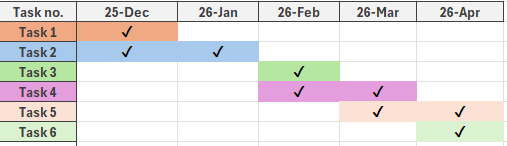
\includegraphics[width=\textwidth]{workplan.png}
\caption{Gantt Chart for Timeline.}
\label{FIG:workplan}
\end{figure}

%%%%%%%%%%%%%%%%%%%%%%% Chapter 5: Preliminary Literature Review %%%%%%%%%%%%%%%%%%%%%%%%%%%%%
% \chapter{Preliminary Literature Review}
% Summarize existing literature related to the topic and identify knowledge gaps.

% \begin{figure}[h!]
%     \centering
%     \includegraphics[width=0.7\textwidth]{example-image-a} % Replace with your image
%     \caption{Trends in Neural Network Research}
%     \label{fig:neural_trends}
% \end{figure}

%%%%%%%%%%%%%%%%%%%%%%% Chapter 6: Methodology %%%%%%%%%%%%%%%%%%%%%%%%%%%%%
% \chapter{Methodology}
% Describe the research methods and tools. Include any relevant equations or algorithms.

% \section{Mathematical Representation}
% For example, the gradient descent algorithm is given by:
% \begin{equation}
%     x_{k+1} = x_k - \alpha \nabla f(x_k)
%     \label{eq:gradient_descent}
% \end{equation}

% %%%%%%%%%%%%%%%%%%%%%%% Chapter 7: Expected Outcomes %%%%%%%%%%%%%%%%%%%%%%%%%%%%%
% \chapter{Expected Outcomes}
% Outline the anticipated results of the research. For example, Table~\ref{tab:expected_outcomes} summarizes the key outcomes.

% \begin{table}[h!]
%     \caption{Expected Outcomes}
%     \centering
%     \begin{tabular}{|c|c|}
%         \hline
%         Outcome & Description \\ \hline
%         Improved Accuracy & Better performance of neural networks. \\ \hline
%         Scalability Insights & Insights into hardware-software interactions. \\ \hline
%     \end{tabular}
%     \label{tab:expected_outcomes}
% \end{table}

% %%%%%%%%%%%%%%%%%%%%%%% Chapter 8: Working Schedule %%%%%%%%%%%%%%%%%%%%%%%%%%%%%
% \chapter{Working Schedule}
% Provide a timeline for completing the research. For example:

% \begin{table}[h!]
%     \caption{Proposed Work Schedule}
%     \centering
%     \begin{tabular}{|c|c|}
%         \hline
%         Task & Timeline \\ \hline
%         Literature Review & Month 1-2 \\ \hline
%         Data Collection & Month 3-5 \\ \hline
%         Analysis & Month 6-7 \\ \hline
%         Documentation & Month 8-9 \\ \hline
%     \end{tabular}
%     \label{tab:work_schedule}
% \end{table}

% %%%%%%%%%%%%%%%%%%%%%%% References %%%%%%%%%%%%%%%%%%%%%%%%%%%%%

\bibliographystyle{IEEEtran}
\bibliography{references} % Replace with the actual .bib file path

\end{document}